\section{Pre-training}

The base model of Kimi K2 is a trillion-parameter mixture-of-experts (MoE) transformer~\citep{transformer} model, pre-trained on 15.5 trillion high-quality tokens. Given the increasingly limited availability of high-quality human data, we posit that token efficiency is emerging as a critical coefficient in the scaling of large language models. To address this, we introduce a suite of pre-training techniques explicitly designed for maximizing token efficiency. Specifically, we employ the token-efficient Muon optimizer~\citep{jordan2024muon,liu2025muon} and mitigate its training instabilities through the introduction of QK-Clip. Additionally, we incorporate synthetic data generation to further squeeze the intelligence out of available high-quality tokens. The model architecture follows an ultra-sparse MoE with multi-head latent attention~(MLA) similar to DeepSeek-V3~\citep{deepseekai2024deepseekv3technicalreport} , derived from empirical scaling law analysis. The underlying infrastructure is built to optimize both training efficiency and research efficiency.







\subsection{MuonClip: Stable Training with Weight Clipping}



We train Kimi K2 using the token-efficient Muon optimizer~\citep{jordan2024muon}, incorporating weight decay and consistent update RMS scaling~\citep{liu2025muon}. Experiments in our previous work Moonlight~\citep{liu2025muon} show that, under the same compute budget and model size --- and therefore the same amount of training data --- Muon substantially outperforms AdamW~\citep{adam2015kingma, loshchilov2018decoupled}, making it an effective choice for improving token efficiency in large language model training.

\paragraph{Training instability when scaling Muon}
Despite its efficiency, scaling up Muon training reveals a challenge: training instability due to exploding attention logits, an issue that occurs more frequently with Muon but less with AdamW in our experiments. Existing mitigation strategies are insufficient. For instance, logit soft-cap~\citep{team2024gemma} directly clips the attention logits, but the dot products between queries and keys can still grow excessively before capping is applied. On the other hand, Query-Key Normalization (QK-Norm)~\citep{dehghani2023scaling,wortsman2309small} is not applicable to multi-head latent attention (MLA), because its Key matrices are not fully materialized during inference.


\paragraph{Taming Muon with QK-Clip}
To address this issue, we propose a novel weight-clipping mechanism \textit{QK-Clip} to explicitly constrain attention logits. QK-Clip works by rescaling the query and key projection weights post-update to bound the growth of attention logits.
 
Let the input representation of a transformer layer be $\mathbf X$. For each attention head $h$, its query, key, and value projections are computed as
\[
\mathbf{Q}^{h} = \mathbf X \mathbf W_q^{h}, \quad
\mathbf K^{h} = \mathbf X \mathbf W_k^{h}, \quad
\mathbf V^{h} = \mathbf X \mathbf W_v^{h}.
\]
where $\mathbf W_q, \mathbf W_k, \mathbf W_v$ are model parameters. The attention output is:

\[
\mathbf O^{h} = \operatorname{softmax}\left( \frac{1}{\sqrt{d}} \mathbf Q^{h} \mathbf K^{h\top} \right) \mathbf V^{h}.
\]

We define the max logit, a per-head scalar, as the maximum input to softmax in this batch $B$:
\[
S_{\max}^{h} = \frac{1}{\sqrt{d}} \max_{\mathbf X \in B} \max_{i,j} \mathbf Q_i^{h} \mathbf K_j^{h\top} 
\]
where $i,j$ are indices of different tokens in a training sample $\mathbf X$.



The core idea of QK-Clip is to rescale $\mathbf W_k, \mathbf W_q$ whenever $S_{\max}^{h}$ exceeds a target threshold $\tau$. Importantly, this operation does not alter the forward/backward computation in the current step --- we merely use the max logit as a guiding signal to determine the strength to control the weight growth.

A naïve implementation clips all heads at the same time:
\begin{equation*}
  \mathbf W_q^{h} \gets \gamma^{\alpha} \mathbf  W_q^{h} \qquad
  \mathbf W_k^{h} \gets  \gamma^{1-\alpha} \mathbf W_k^{h}
\end{equation*}
where $\gamma = \min(1, \tau / S_{\max})$ with $S_{\max} = \max_h S_{\max}^{h}$, and $\alpha$ is a balancing parameter typically set to $0.5$, applying equal scaling to queries and keys. 

However, we observe that in practice, only a small subset of heads exhibit exploding logits. In order to minimize our intervention on model training, we determine a per-head scaling factor $\gamma_h = \min(1, \tau / S_{\max}^h) $, and opt to apply per-head QK-Clip. Such clipping is straightforward for regular multi-head attention (MHA). For MLA, we apply clipping only on unshared attention head components:

\begin{itemize}
\item $\textbf{q}^{C}$ and $\textbf{k}^{C}$ (head-specific components): each scaled by $\sqrt{\gamma_h}$ 
\item $\textbf{q}^{R}$ (head-specific rotary): scaled by $\gamma_h$,
\item $\textbf{k}^{R}$ (shared rotary): left untouched to avoid effect across heads.
\end{itemize}

\begin{algorithm}[t]
\caption{MuonClip Optimizer}
\label{alg:muonclip}
\begin{algorithmic}[1]
\For{each training step $t$}
   \State \textcolor{gray}{// 1. Muon optimizer step}
   \For{each weight $\mathbf W\in\mathbb{R}^{n\times m}$}
        \State $\mathbf M_t = \mu \mathbf M_{t-1} + \mathbf G_t$ \Comment{$\mathbf M_0 = \mathbf 0$, $\mathbf G_t$ is the grad of $\mathbf W_t$, $\mu$ is momentum}
        \State $\mathbf O_t = \operatorname{Newton-Schulz}(\mathbf M_t)\cdot \sqrt{\max(n,m)}\cdot 0.2$ \Comment{Match Adam RMS}
        \State $\mathbf W_t = \mathbf W_{t-1} - \eta \bigl(\mathbf O_t + \lambda \mathbf W_{t-1}\bigr)$ \Comment{learning rate $\eta$, weight decay $\lambda$}
   \EndFor
   \State \textcolor{gray}{// 2. QK-Clip}
   \For{each attention head $h$ in every attention layer of the model}
       \State Obtain $S_{\max}^{h}$ already computed during forward
       \If{$S_{\max}^{h} > \tau$}
           \State $\gamma \gets \tau / S_{\max}^{h}$
           \State $\mathbf W_{qc}^{h} \gets \mathbf W_{qc}^{h} \cdot \sqrt{\gamma}$
           \State $\mathbf W_{kc}^{h} \gets \mathbf W_{kc}^{h} \cdot \sqrt{\gamma}$
           \State $\mathbf W_{qr}^{h} \gets \mathbf W_{qr}^{h} \cdot \gamma$
       \EndIf
   \EndFor
\EndFor
\end{algorithmic}
\end{algorithm}












\begin{figure}[htbp]
  \centering
  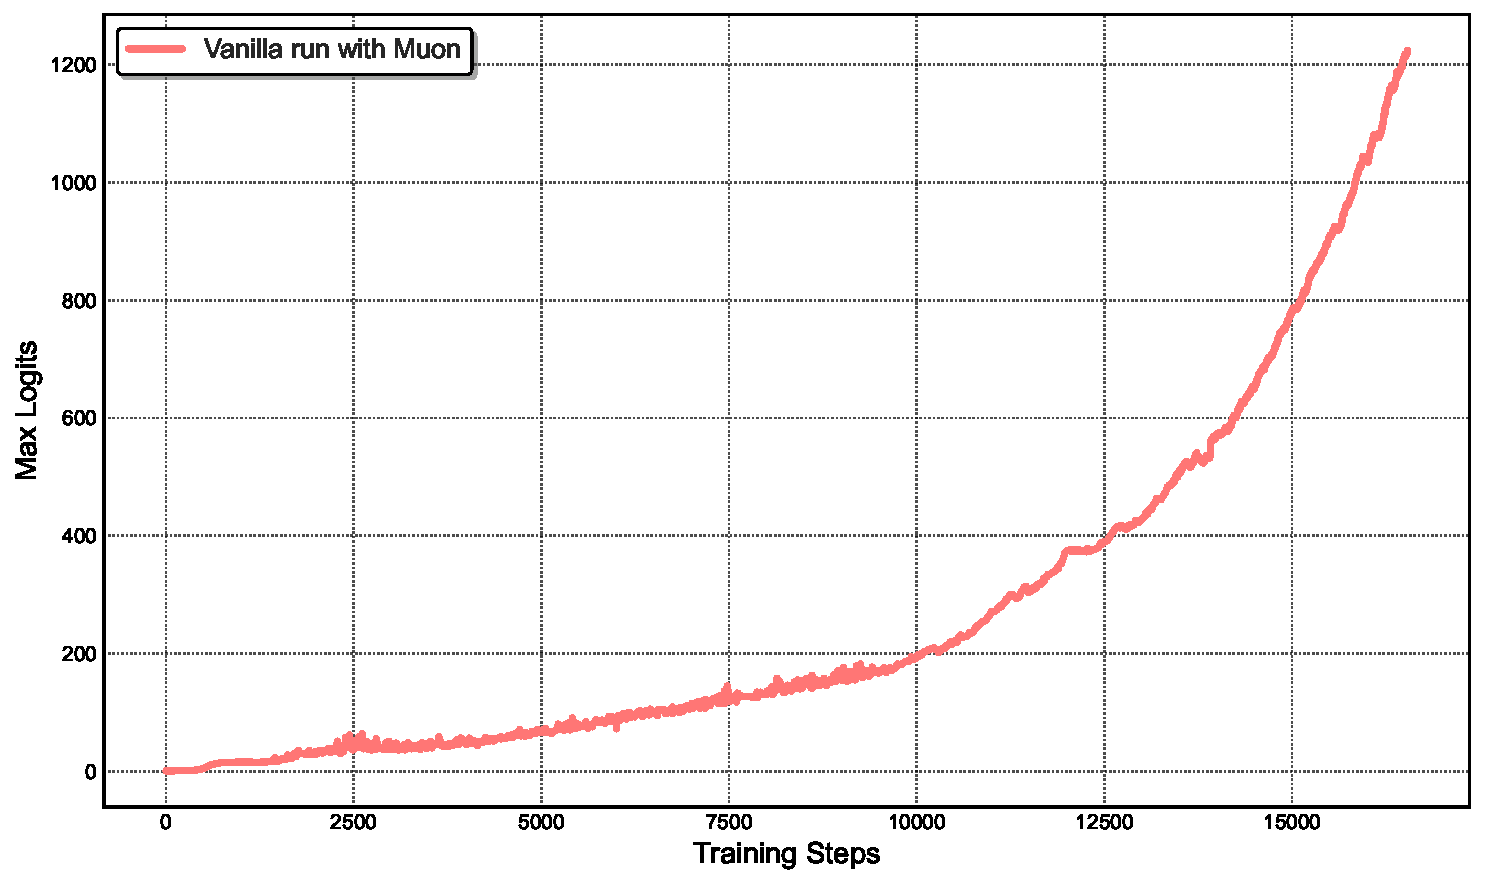
\includegraphics[width=.48\linewidth]{figures/muon-MN-max-logits.pdf}
  \hfill
  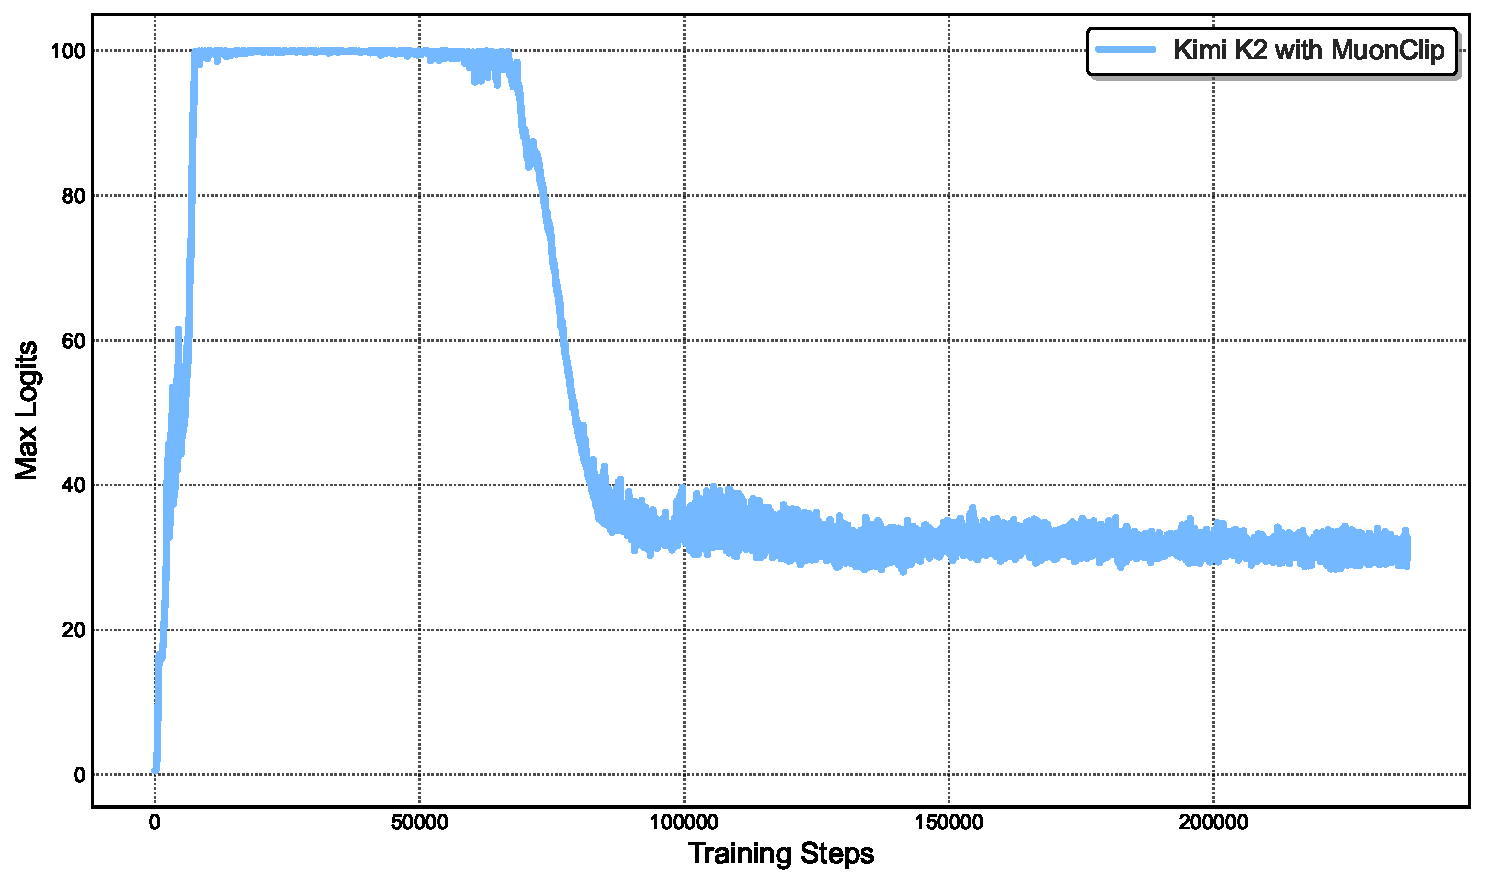
\includegraphics[width=.48\linewidth]{figures/muon-K2-max-logits.pdf}
  

  \caption{Left: During a mid-scale training run, attention logits rapidly exceed 1000, which could lead to potential numerical instabilities and even training divergence.  Right: Maximum logits for Kimi K2 with MuonClip and $\tau$ = 100 over the entire training run. 
  The max logits rapidly increase to the capped value of 100, and only decay to a stable range after approximately 30\% of the training steps, demonstrating the effective regulation effect of QK-Clip.}

  \label{fig:mini_muonclip}
\end{figure}

\paragraph{MuonClip: The New Optimizer}

We integrate Muon with weight decay, consistent RMS matching, and QK-Clip into a single optimizer, which we refer to as \textbf{MuonClip} (see Algorithm~\ref{alg:muonclip}).

We demonstrate the effectiveness of MuonClip from several scaling experiments. First, we train a mid-scale 9B activated and 53B total parameters Mixture-of-Experts (MoE) model using the vanilla Muon. As shown in Figure~\ref{fig:mini_muonclip} (Left), we observe that the maximum attention logits quickly exceed a magnitude of 1000, showing that attention logits explosion is already evident in Muon training to this scale. Max logits at this level usually result in instability during training, including significant loss spikes and occasional divergence.

Next, we demonstrate that QK-Clip does not degrade model performance and confirm that the MuonClip optimizer preserves the optimization characteristics of Muon without adversely affecting the loss trajectory. A detailed discussion of the experiment designs and findings is provided in the Appendix~\ref{sec:qkclip_harmless}.

Finally, we train Kimi K2, a large-scale MoE model, using MuonClip with $\tau = 100$ and monitor the maximum attention logits throughout the training run (Figure~\ref{fig:mini_muonclip} (Right)). Initially, the logits are capped at 100 due to QK-Clip. Over the course of training, the maximum logits gradually decay to a typical operating range without requiring any adjustment to $\tau$. Importantly, the training loss remains smooth and stable, with no observable spikes, as shown in Figure~\ref{fig:kimi-loss-curve}, validating that MuonClip provides robust and scalable control over attention dynamics in large-scale language model training.




\begin{figure}[htb]
    \centering
    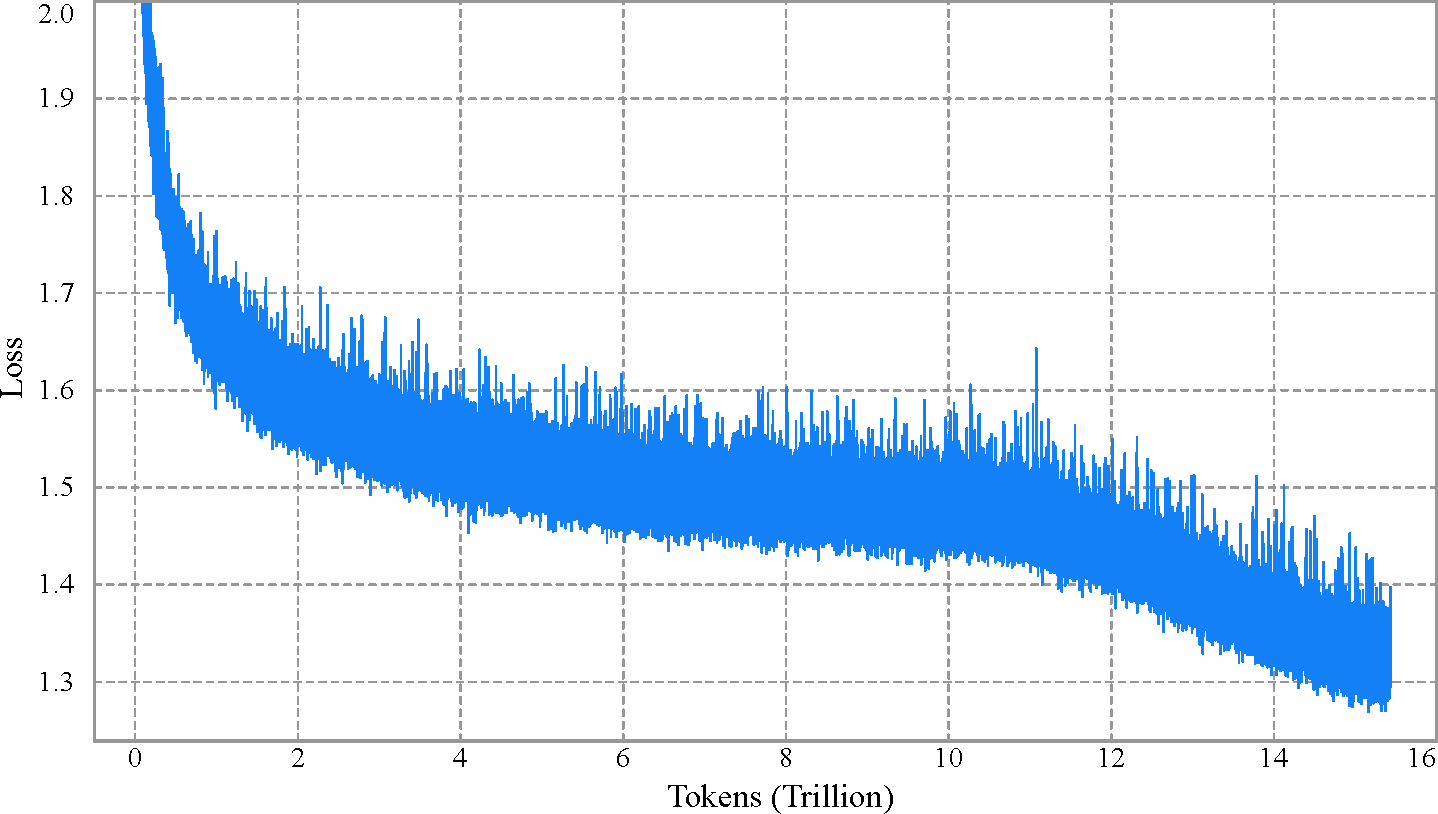
\includegraphics[width=0.7\textwidth]{figures/loss_vs_tokens_white.pdf}
    \caption{Per-step training loss curve of Kimi K2, \textbf{without smoothing or sub-sampling}. It shows no spikes throughout the entire training process. Note that we omit the very beginning of training for clarity.} 
    \label{fig:kimi-loss-curve}
\end{figure}








\subsection{Pre-training Data: Improving Token Utility with Rephrasing}

Token efficiency in pre-training refers to how much performance improvement is achieved for each token consumed during training. Increasing token utility—the effective learning signal each token contributes—enhances the per-token impact on model updates, thereby directly improving token efficiency. 
This is particularly important when the supply of high-quality tokens is limited and must be maximally leveraged. A naive approach to increasing token utility is through repeated exposure to the same tokens, which can lead to overfitting and reduced generalization.

A key advancement in the pre-training data of Kimi K2 over Kimi K1.5 is the introduction of a synthetic data generation strategy to increase token utility. Specifically, a carefully designed rephrasing pipeline is employed to amplify the volume of high-quality tokens without inducing significant overfitting. In this report, we describe two domain-specialized rephrasing techniques—targeted respectively at the Knowledge and Mathematics domains—that enable this controlled data augmentation.



\paragraph{Knowledge Data Rephrasing}
Pre-training on natural, knowledge-intensive text presents a trade-off: a single epoch is insufficient for comprehensive knowledge absorption, while multi-epoch repetition yields diminishing returns and increases the risk of overfitting. To improve the token utility of high-quality knowledge tokens, we propose a synthetic rephrasing framework composed of the following key components:

\begin{itemize}
    \item \textbf{Style- and perspective-diverse prompting:} Inspired by WRAP~\citep{maini2024rephrasingwebrecipecompute}, we apply a range of carefully engineered prompts to enhance linguistic diversity while maintaining factual integrity. These prompts guide a large language model to generate faithful rephrasings of the original texts in varied styles and from different perspectives.
    
    \item \textbf{Chunk-wise autoregressive generation:} To preserve global coherence and avoid information loss in long documents, we adopt a chunk-based autoregressive rewriting strategy. Texts are divided into segments, rephrased individually, and then stitched back together to form complete passages. This method mitigates implicit output length limitations that typically exist with LLMs. An overview of this pipeline is presented in Figure~\ref{fig:rephrase_pipeline}.

    \item \textbf{Fidelity verification:} To ensure consistency between original and rewritten content, we perform fidelity checks that compare the semantic alignment of each rephrased passage with its source. This serves as an initial quality control step prior to training.
\end{itemize}

We compare data rephrasing with multi-epoch repetition by testing their corresponding accuracy on SimpleQA.
We experiment with an early checkpoint of K2 and evaluate three training strategies: (1) repeating the original dataset for 10 epochs, (2) rephrasing the data once and repeating it for 10 epochs, and (3) rephrasing the data 10 times with a single training pass. 
As shown in Table~\ref{tab:rewrites_epochs_f1}, the accuracy consistently improves across these strategies, demonstrating the efficacy of our rephrasing-based augmentation. We extended this method to other large-scale knowledge corpora and observed similarly encouraging results, and each corpora is rephrased at most twice.


\begin{table}[htbp]
\centering
\caption{SimpleQA Accuracy under three rephrasing-epoch configurations}
\label{tab:rewrites_epochs_f1}
\begin{tabular}{ccc}
\toprule
\# Rephrasings & \# Epochs & SimpleQA Accuracy \\
\midrule
0 (raw wiki-text) & 10 & 23.76 \\
1            & 10 & 27.39 \\
10           & 1  & 28.94 \\
\bottomrule
\end{tabular}
\end{table}



\begin{figure}[t]
\centering
\begin{minipage}[t]{0.8\textwidth}
  \centering
  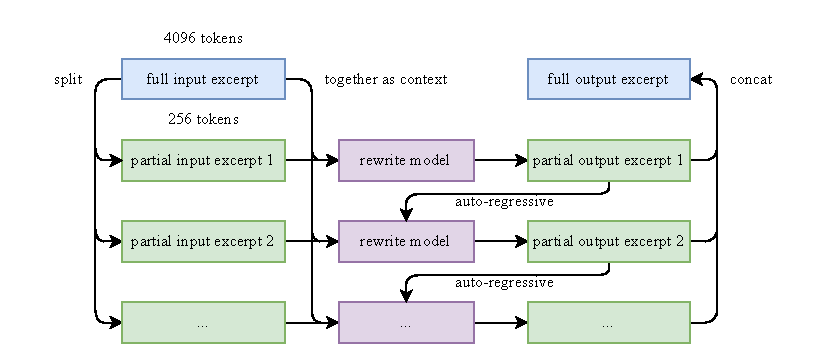
\includegraphics[width=\linewidth]{figures/synthetic_data_rephrase.pdf}
  \caption{Auto-regressive chunk-wise rephrasing pipeline for long input excerpts. The input is split into smaller chunks with preserved context, rewritten sequentially, and then concatenated into a full rewritten passage. }
  \label{fig:rephrase_pipeline}
\end{minipage}\hfill
\end{figure}

    
\paragraph{Mathematics Data Rephrasing} To enhance mathematical reasoning capabilities, we rewrite high-quality mathematical documents into a ``learning-note'' style, following the methodology introduced in SwallowMath~\citep{fujii2025rewritingpretrainingdataboosts}. In addition, we increased data diversity by translating high-quality mathematical materials from other languages into English.

Although initial experiments with rephrased subsets of our datasets show promising results, the use of synthetic data as a strategy for continued scaling remains an active area of investigation. Key challenges include generalizing the approach to diverse source domains without compromising factual accuracy, minimizing hallucinations and unintended toxicity, and ensuring scalability to large-scale datasets.

\paragraph{Pre-training Data Overall} The Kimi K2 pre-training corpus comprises 15.5 trillion tokens of curated, high-quality data spanning four primary domains: Web Text, Code, Mathematics, and Knowledge. Most data processing pipelines follow the methodologies outlined in Kimi K1.5~\citep{team2025kimi}. For each domain, we performed rigorous correctness and quality validation and designed targeted data experiments to ensure the curated dataset achieved both high diversity and effectiveness.












\subsection{Model Architecture}
Kimi K2 is a 1.04 trillion-parameter Mixture-of-Experts (MoE) transformer model with 32 billion activated parameters. The architecture follows a similar design to DeepSeek-V3~\citep{deepseekai2024deepseekv3technicalreport} , employing Multi-head Latent Attention (MLA)~\citep{liu2024deepseek} as the attention mechanism, with a model hidden dimension of 7168 and an MoE expert hidden dimension of 2048. Our scaling law analysis reveals that continued increases in sparsity yield substantial performance improvements, which motivated us to increase the number of experts to 384, compared to 256 in DeepSeek-V3. To reduce computational overhead during inference, we cut the number of attention heads to 64, as opposed to 128 in DeepSeek-V3. Table~\ref{tab:k2_arch_comparison} presents a detailed comparison of architectural parameters between Kimi K2 and DeepSeek-V3.

\begin{table}[htbp]
\centering
\caption{Architectural comparison between Kimi K2 and DeepSeek-V3}
\label{tab:k2_arch_comparison}
\begin{tabular}{lccc}
\toprule
  & \textbf{DeepSeek-V3} & \textbf{Kimi K2} & \textbf{$\Delta$} \\
\midrule
\#Layers & 61 & 61 & = \\
Total Parameters & 671B & 1.04T & $\uparrow$ 54\% \\
Activated Parameters & 37B & 32.6B & $\downarrow$ 13\% \\
Experts (total) & 256 & 384 & $\uparrow$ 50\% \\
Experts Active per Token & 8 & 8 & = \\
Shared Experts & 1 & 1 & = \\
Attention Heads & 128 & 64 & $\downarrow$ 50\% \\
Number of Dense Layers & 3 & 1 & $\downarrow$ 67\% \\
Expert Grouping & Yes & No  & - \\
\bottomrule
\end{tabular}
\end{table}


\paragraph{Sparsity Scaling Law}
We develop a sparsity scaling law tailored for the Mixture-of-Experts (MoE) model family using Muon. Sparsity is defined as the ratio of the total number of experts to the number of activated experts. Through carefully controlled small-scale experiments, we observe that --- under a fixed number of activated parameters (i.e., constant FLOPs) --- increasing the total number of experts (i.e., increasing sparsity) consistently lowers both the training and validation loss, thereby enhancing overall model performance (Figure~\ref{fig:scaling-law}). Concretely, under the compute-optimal sparsity scaling law, achieving the same validation loss of 1.5, sparsity 48 reduces FLOPs by 1.69×, 1.39×, and 1.15× compared to sparsity levels 8, 16, and 32, respectively.
Though increasing sparsity leads to better performance, this gain comes with increased infrastructure complexity. To balance model performance with cost, we adopt a sparsity of 48 for Kimi K2, activating 8 out of 384 experts per forward pass.

\begin{figure}[htbp]
\centering
\begin{minipage}[t]{0.48\textwidth}
  \centering

  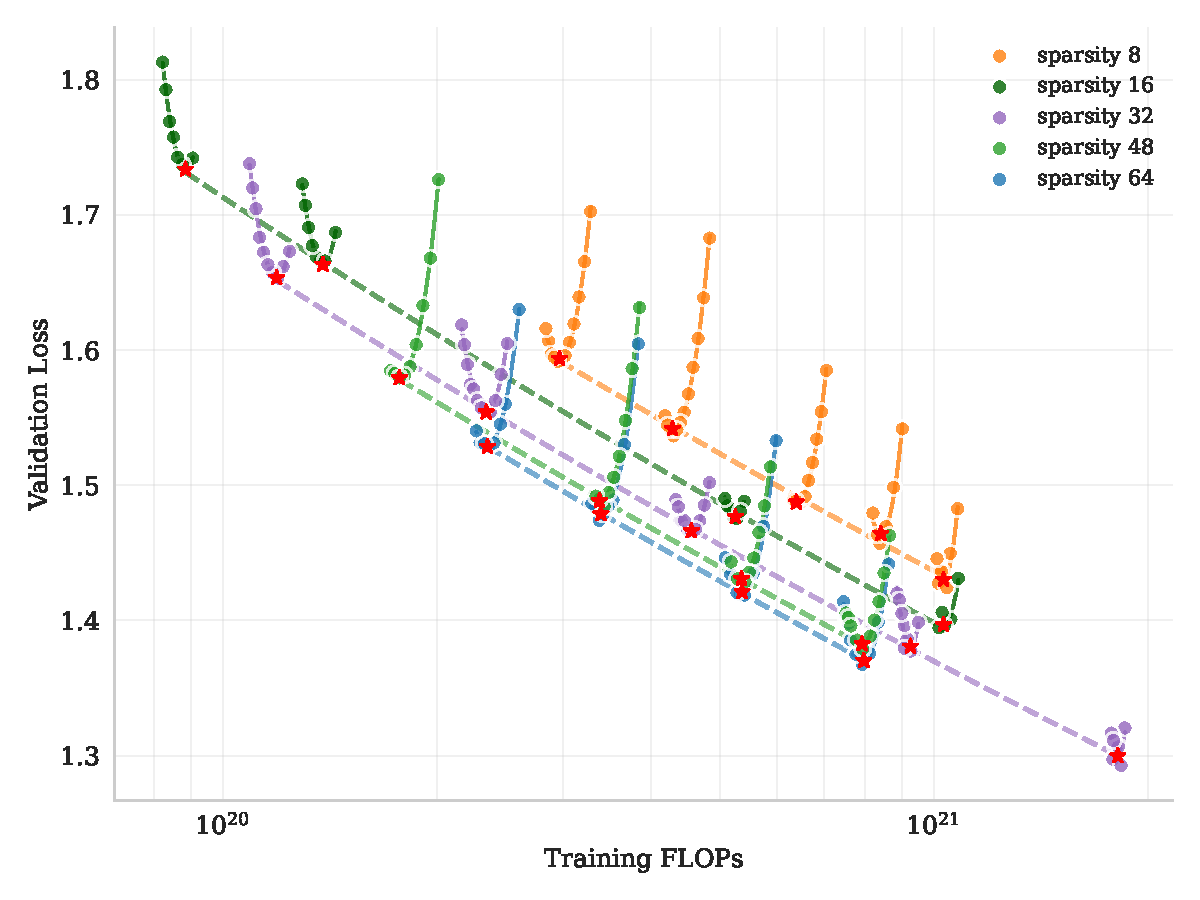
\includegraphics[width=\linewidth]{figures/scaling_law_validation_loss}
  \caption{Sparsity Scaling Law. Increasing sparsity leads to improved model performance. We fixed the number of activated experts to 8 and the number of shared experts to 1, and varied the total number of experts, resulting in models with different sparsity levels.}
  \label{fig:scaling-law}
  
  
\end{minipage}\hfill
\begin{minipage}[t]{0.48\textwidth}
  \centering

  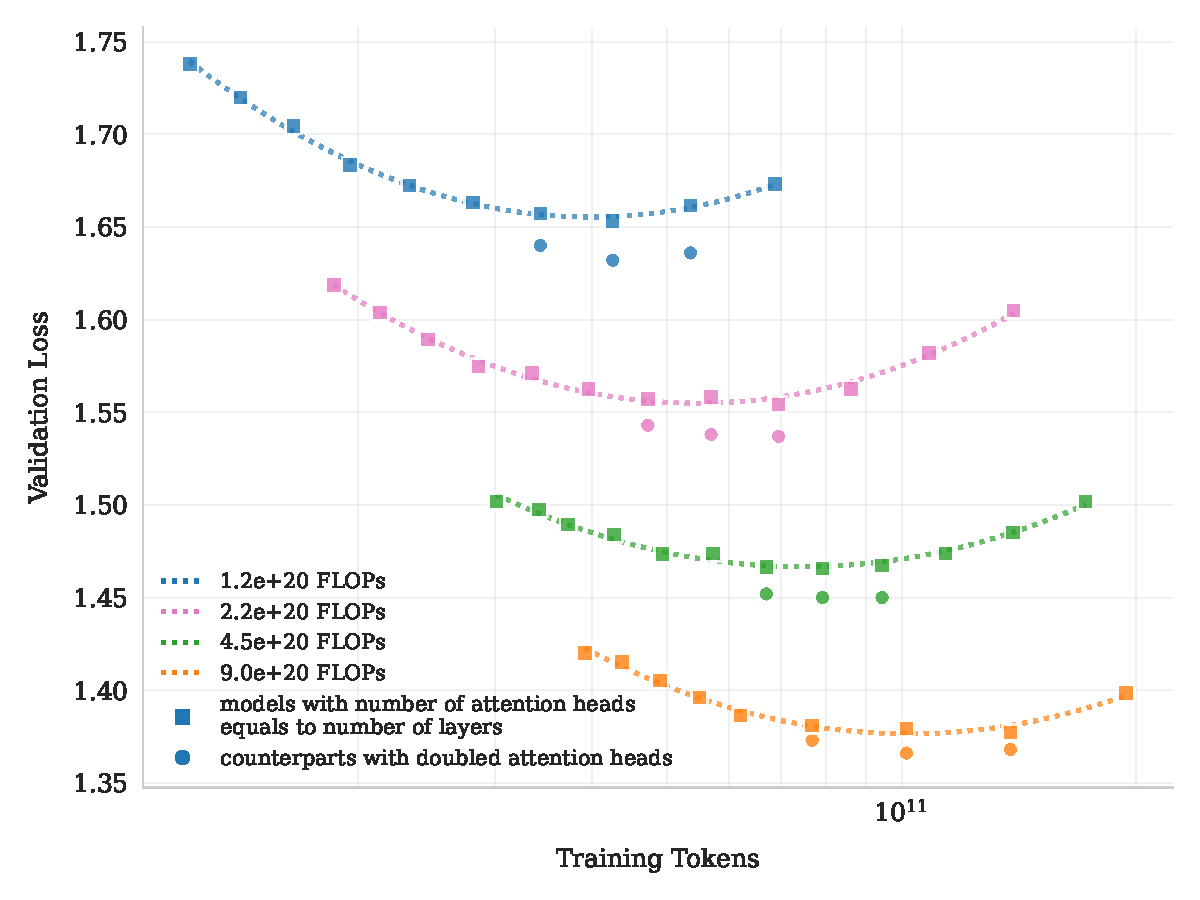
\includegraphics[width=\linewidth]{figures/doubleQheads}
  \caption{Scaling curves for models with number of attention heads equals to number of layers and their counterparts with doubled attention heads. Doubling the number of attention heads leads to a reduction in validation loss of approximately $0.5\%$ to $1.2\%$.}
  \label{fig:doubleQheads}
 
\end{minipage}
\end{figure}

\paragraph{Number of Attention Heads}

DeepSeek-V3~\citep{deepseekai2024deepseekv3technicalreport}  sets the number of attention heads to roughly twice the number of model layers to better utilize memory bandwidth and enhance computational efficiency. 
However, as the context length increases, doubling the number of attention heads leads to significant inference overhead, reducing efficiency at longer sequence lengths. This becomes a major limitation in agentic applications, where efficient long context processing is essential.
For example, with a sequence length of 128k, increasing the number of attention heads from 64 to 128, while keeping the total expert count fixed at 384, leads to an 83\% increase in inference FLOPs.
To evaluate the impact of this design, we conduct controlled experiments comparing configurations where the number of attention heads equals the number of layers against those with double number of heads, under varying training FLOPs. Under iso-token training conditions, we observe that doubling the attention heads yields only modest improvements in validation loss (ranging from 0.5\% to 1.2\%) across different compute budgets (Figure~\ref{fig:doubleQheads}).
Given that sparsity 48 already offers strong performance, the marginal gains from doubling attention heads do not justify the inference cost. Therefore we choose to 64 attention heads.

\subsection{Training Infrastructure}
\subsubsection{Compute Cluster}

Kimi K2 was trained on a cluster equipped with NVIDIA H800 GPUs. Each node in
the H800 cluster contains 2 TB RAM and 8 GPUs connected by NVLink and NVSwitch within nodes. Across
different nodes, $\text{8}\!\times\!\text{400}~\text{Gbps}$ RoCE interconnects are utilized to facilitate communications.

\subsubsection{Parallelism for Model Scaling}

Training of large language models often progresses under dynamic resource availability. Instead of optimizing one parallelism strategy that's only applicable under specific amount of resources, we pursue a flexible strategy that allows Kimi K2 to be trained on any number of nodes that is a multiple of 32.
Our strategy leverages a combination of 16-way Pipeline Parallelism (PP) with virtual stages~\citep{huang2019gpipe, narayanan2021efficient, lamy2023breadth, qi2023zero, Liu_2023, harlap2018pipedream}, 16-way Expert Parallelism (EP)~\citep{lepikhin2020gshard}, and ZeRO-1 Data Parallelism~\citep{rajbhandari2020zero}.

Under this setting, storing the model parameters in BF16 and their gradient accumulation buffer in FP32 requires approximately 6 TB of GPU memory, distributed over a model-parallel group of 256 GPUs. 
Placement of optimizer states depends on the training configurations. When the total number of training nodes is large, the optimizer states are distributed, reducing its per-device memory footprint to a negligible level. When the total number of training nodes is small (e.g., 32), we can offload some optimizer states to CPU. 

This approach allows us to reuse an identical parallelism configuration for both small- and large-scale experiments, while letting each GPU hold approximately 30 GB of GPU memory for all states. The rest of the GPU memory are used for activations, as described in Sec.~\ref{sec:act_reduction}.
Such a consistent design is important for research efficiency, as it simplifies the system and substantially accelerates experimental iteration.

\paragraph{EP communication overlap with interleaved 1F1B}

By increasing the number of warm-up micro-batches, we can overlap EP all-to-all communication with computation under the standard interleaved 1F1B schedule \citep{harlap2018pipedream, narayanan2021efficient}. 
In comparison, DualPipe~\citep{deepseekai2024deepseekv3technicalreport} doubles the memory required for parameters and gradients, necessitating an increase in parallelism to compensate.
Increasing PP introduces more bubbles, while increasing EP, as discussed below, incurs higher overhead.
The additional costs are prohibitively high for training a large model with over 1 trillion parameters and thus we opted not to use DualPipe. 

However, interleaved 1F1B splits the model into more stages, introducing non-trivial PP communication overhead. To mitigate this cost, we decouple the weight-gradient computation from each micro-batch's backward pass and execute it in parallel with the corresponding PP communication.
Consequently, all PP communications can be effectively overlapped except for the warm-up phase.


\paragraph{Smaller EP size}

To ensure full computation-communication overlap during the 1F1B stage, the reduced attention computation time in K2~(which has 64 attention heads compared to 128 heads in DeepSeek-V3) necessitates minimizing the time of EP operations. 
This is achieved by adopting the smallest feasible EP parallelization strategy, specifically EP = 16.
Utilizing a smaller EP group also relaxes expert-balance constraints, allowing for near-optimal speed to be achieved without further tuning.


\subsubsection{Activation Reduction}
\label{sec:act_reduction}

After reserving space for parameters, gradient buffers, and optimizer states, the remaining GPU memory on each device is insufficient to hold the full MoE activations. To ensure the activation memory fits within the constraints, especially for the initial pipeline stages that accumulate the largest activations during the 1F1B warm-up phase, the following techniques are employed.


\paragraph{Selective recomputation}

Recomputation is applied to inexpensive, high-footprint stages, including \texttt{LayerNorm}, \texttt{SwiGLU}, and \texttt{MLA} up-projections~\citep{deepseekai2024deepseekv3technicalreport}.
Additionally, \texttt{MoE} down-projections are recomputed during training to further reduce activation memory. While optional, this recomputation maintains adequate GPU memory, preventing crashes caused by expert imbalance in early training stages.

\paragraph{FP8 storage for insensitive activations}

Inputs of \texttt{MoE} up-projections and \texttt{SwiGLU} are compressed to FP8-E4M3 in 1$\times$ 128 tiles with FP32 scales. Small-scale experiments show no measurable loss increase. Due to potential risks of performance degradation that we observed during preliminary study, we do not apply FP8 in computation.

\begin{figure}
    \centering
    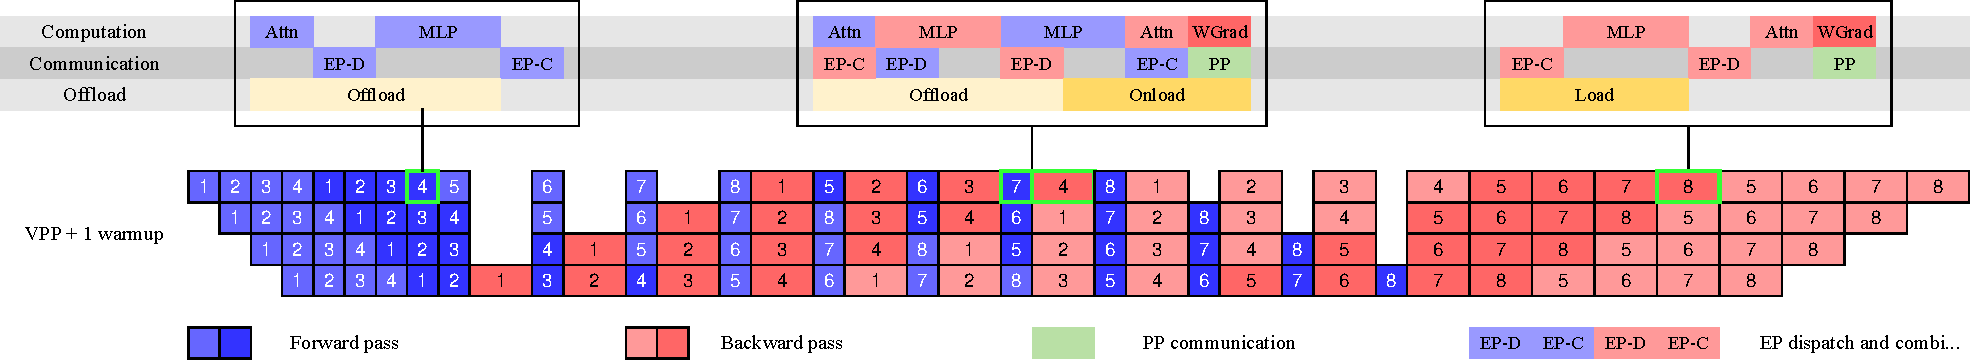
\includegraphics[width=1\linewidth]{figures/3x_stream.pdf}
    \caption{Computation, communication and offloading overlapped in different PP phases.}
    \label{fig:3x_stream}
\end{figure}
\paragraph{Activation CPU offload}

All remaining activations are offloaded to CPU RAM. A copy engine is responsible for streaming the offload and onload, overlapping with both computation and communication kernels. During the 1F1B phase, we offload the forward activations of the previous micro-batch while prefetching the backward activations of the next. The warm-up and cool-down phases are handled similarly and the overall pattern is shown in Figure~\ref{fig:3x_stream}. Although offloading may slightly affect EP traffic due to PCIe traffic congestion, our tests show that EP communication remains fully overlapped.



\subsection{Training recipe}

We pre-trained the model with a 4,096-token context window using the MuonClip optimizer (Algorithm~\ref{alg:muonclip}) and the WSD learning rate schedule~\citep{hu2024minicpm}, processing a total of 15.5T tokens. 
The first 10T tokens were trained with a constant learning rate of 2e-4 after a 500-step warm-up,
followed by 5.5T tokens with a cosine decay from 2e-4 to 2e-5. 
Weight decay was set to 0.1 throughout, and the global batch size was held at 67M tokens. The overall training curve is shown in Figure~\ref{fig:kimi-loss-curve}.

Towards the end of pre-training, we conducted an annealing phase followed by a long-context activation stage. The batch size was kept constant at 67M tokens, while the learning rate was decayed from 2e-5 to 7e-6. In this phase, the model was trained on 400 billion tokens with a 4k sequence length, followed by an additional 60 billion tokens with a 32k sequence length. To extend the context window to 128k, we employed the YaRN method~\citep{peng2023yarn}.








    





